
\documentclass[12pt,a4paper]{article}

\usepackage[a4paper,margin=1in]{geometry}
\usepackage{graphicx}
\usepackage{booktabs}
\usepackage{amsmath,amssymb}
\usepackage{float}
\usepackage{hyperref}
\usepackage{xcolor}
\usepackage{listings}
\usepackage{enumitem}
\usepackage{fancyhdr}
\usepackage{longtable}

\hypersetup{colorlinks=true,linkcolor=blue,urlcolor=blue}

\pagestyle{fancy}
\fancyhf{}
\lhead{ICS1512}
\rhead{Machine Learning Algorithms Laboratory}
\cfoot{\thepage}

\begin{document}

\begin{tabular}{|p{4cm}|p{11cm}|}
\hline
Experiment No. & 3 \\ \hline
Experiment Title & Regression Analysis using Linear and Regularized Models
\footnote{\textbf{GitHub Repository: }\url{https://github.com/Barath-j593/ML-assignments}}\\ \hline
Student Name & Barath \\ \hline
Register Number & 3122247001011 \\ \hline
Faculty & Dr. Poreddy Ajay Kumar Reddy \\ \hline
Submission Date & \\ \hline
\end{tabular}

\section{Aim and Objective}
To implement linear and regularized regression models (Linear, Ridge, Lasso, and Elastic
Net) for predicting a continuous target variable -- the sanctioned loan amount -- evaluate
their performance using multiple regression metrics, visualize model behaviour, and analyze
overfitting, underfitting, and bias--variance characteristics.

\section{Dataset Description}
The Kaggle ``Predict Loan Amount Data'' dataset (the standard Loan Prediction dataset) was
used, containing numerical and categorical features related to loan applications, with
\texttt{LoanAmount} as the continuous target variable to be predicted.

\begin{longtable}{|p{6cm}|p{8cm}|}
\hline
Dataset Name & Loan Amount Prediction (Loan Prediction Dataset) \\ \hline
Dataset Source & Kaggle -- \textit{Predict Loan Amount Data} \\ \hline
Original Number of Samples & 614 \\ \hline
Samples after Dropping Missing Target & 592 \\ \hline
Number of Input Features & 10 (6 categorical, 4 numerical) -- expands to 14 after one-hot encoding \\ \hline
Target Variable & LoanAmount (continuous, range 9--700, mean 146.4, std 85.6) \\ \hline
Target Skewness & 2.68 (strongly right-skewed) \\ \hline
Missing Values (Predictors) & Gender (13), Married (2), Dependents (13), Self\_Employed (31), Loan\_Amount\_Term (14), Credit\_History (49) \\ \hline
Train-Test Split & 80:20 (473 train / 119 test), \texttt{random\_state=42} \\ \hline
\end{longtable}

\section{Preprocessing Steps}
\begin{itemize}
\item \textbf{Missing target handling:} 22 rows with a missing \texttt{LoanAmount} value were
dropped, since imputing the regression target itself would fabricate ground truth rather than
genuinely missing predictor information.
\item \textbf{Missing value handling (predictors):} Categorical columns (Gender, Married,
Dependents, Self\_Employed) were imputed with their mode; numerical columns
(Loan\_Amount\_Term, Credit\_History) were imputed with their median.
\item \textbf{Encoding categorical variables:} All six categorical features (Gender, Married,
Dependents, Education, Self\_Employed, Property\_Area) plus Loan\_Status were one-hot encoded
(\texttt{drop="first"} to avoid the dummy-variable trap), expanding 10 raw features into 14
encoded features.
\item \textbf{Standardizing numerical features:} ApplicantIncome, CoapplicantIncome,
Loan\_Amount\_Term, and Credit\_History were standardized (zero mean, unit variance) using
\texttt{StandardScaler}, fit only on the training split and applied to both splits via a
\texttt{ColumnTransformer} inside a \texttt{Pipeline} to prevent data leakage.
\end{itemize}

\section{Implementation Details}
Across the four models were implemented using scikit-learn, wrapped in a single
\texttt{Pipeline} (preprocessing $\rightarrow$ model) to keep preprocessing consistent across
cross-validation folds and the held-out test set.

\begin{itemize}
\item \textbf{Linear Regression:} Trained as the baseline with no regularization and no
hyperparameters to tune.
\item \textbf{Ridge, Lasso, Elastic Net:} Each tuned via \texttt{GridSearchCV} with 5-fold
cross-validation (\texttt{KFold}, \texttt{shuffle=True}, \texttt{random\_state=42}), optimizing
for $R^2$, over the hyperparameter grids specified in the assignment (Ridge:
$\alpha \in \{0.01, 0.1, 1, 10, 100\}$; Lasso: $\alpha \in \{0.001, 0.01, 0.1, 1, 10\}$;
Elastic Net: $\alpha \in \{0.01, 0.1, 1, 10\}$, $\text{l1\_ratio} \in \{0.2, 0.5, 0.8\}$).
\item All four fitted pipelines were then evaluated identically: 5-fold CV metrics on the
training set, and a single held-out evaluation on the untouched 119-row test set.
\end{itemize}

\section{Visualizations}

\begin{figure}[H]
\centering
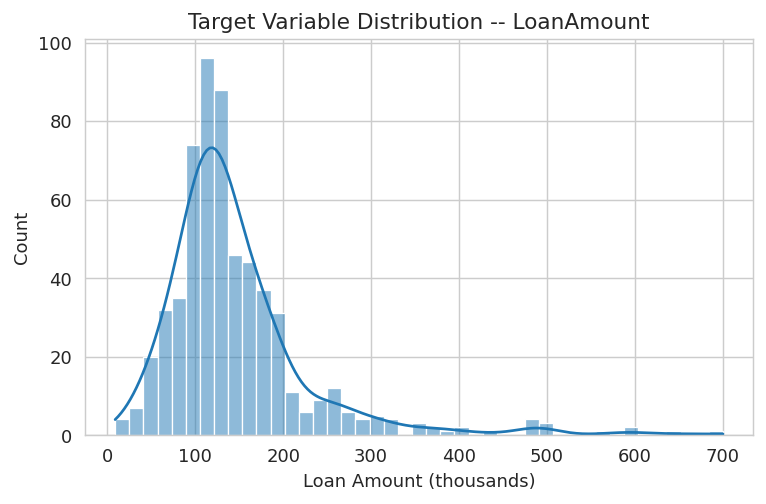
\includegraphics[width=0.6\linewidth]{target_distribution.png}
\caption{Target variable (LoanAmount) distribution}
\end{figure}
\textbf{Inference:} LoanAmount is strongly right-skewed (skewness $\approx 2.68$), with most
sanctioned amounts clustered between 100 and 170 (thousands) and a long tail extending to
700. This skew is a primary driver of the residual pattern seen later, and would justify a
log-transform of the target in a follow-up iteration of this experiment.

\begin{figure}[H]
\centering
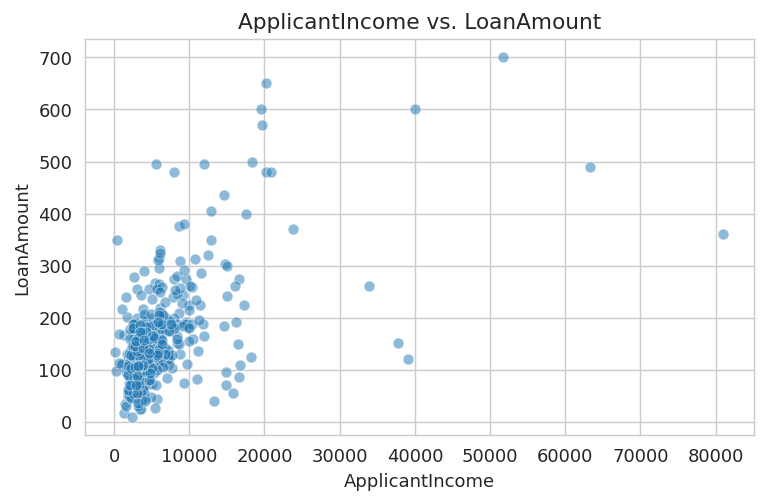
\includegraphics[width=0.55\linewidth]{scatter_ApplicantIncome.png}
\caption{ApplicantIncome vs. LoanAmount}
\end{figure}
\textbf{Inference:} ApplicantIncome shows a moderate positive correlation with LoanAmount
($r \approx 0.57$), the strongest of any single numeric feature, which matches it emerging
as the most heavily weighted feature in every model's coefficients (Section 6). The
relationship is noisy and heteroscedastic -- variance in LoanAmount increases at higher
incomes.

\begin{figure}[H]
\centering
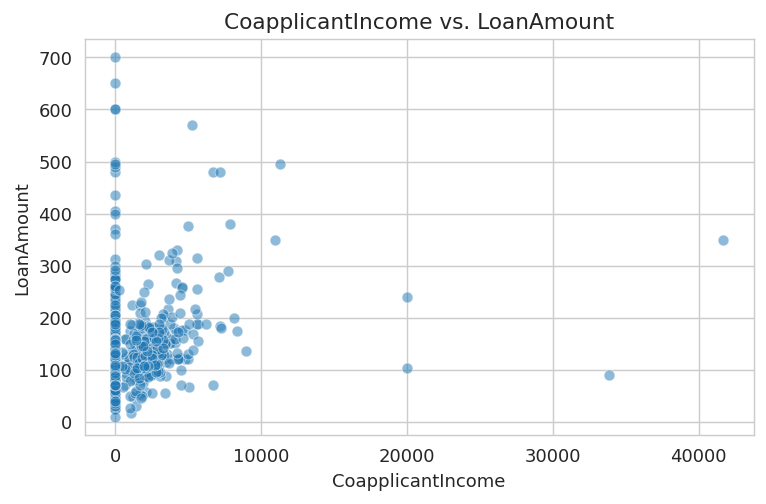
\includegraphics[width=0.55\linewidth]{scatter_CoapplicantIncome.png}
\caption{CoapplicantIncome vs. LoanAmount}
\end{figure}
\textbf{Inference:} CoapplicantIncome is only weakly correlated with LoanAmount ($r \approx
0.19$), and a large cluster of applicants report zero co-applicant income, indicating many
single-applicant loans. This weaker relationship is reflected in a consistently smaller
coefficient for this feature across all four models.

\begin{figure}[H]
\centering
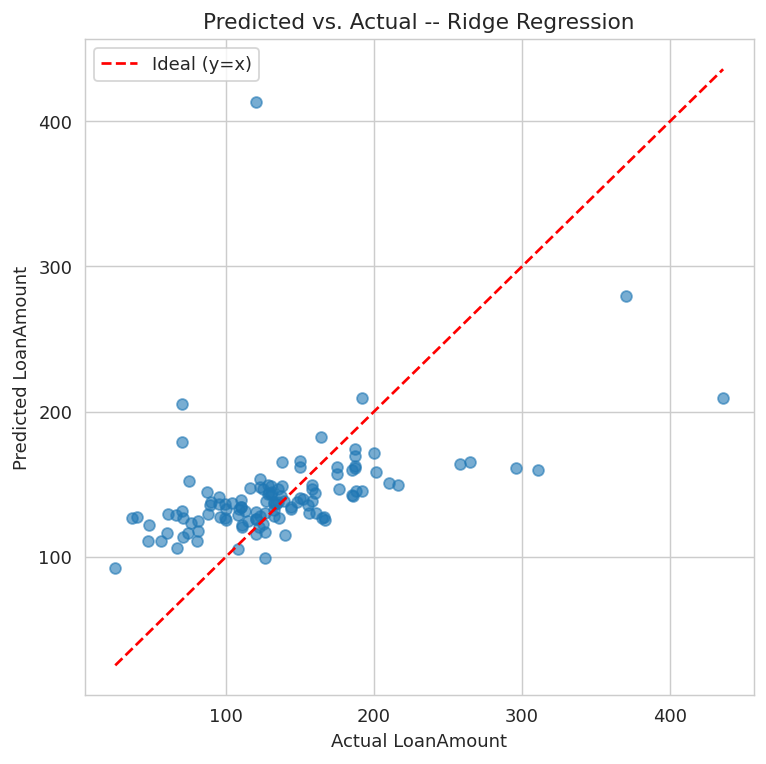
\includegraphics[width=0.55\linewidth]{predicted_vs_actual.png}
\caption{Predicted vs. actual LoanAmount -- best model (Ridge Regression)}
\end{figure}
\textbf{Inference:} Points scatter loosely around the ideal $y=x$ line rather than tracking
it tightly, and the model visibly under-predicts for the highest actual loan amounts (the
right-skew tail), which matches a linear model struggling to capture the more extreme,
rarer high-value loans.

\begin{figure}[H]
\centering
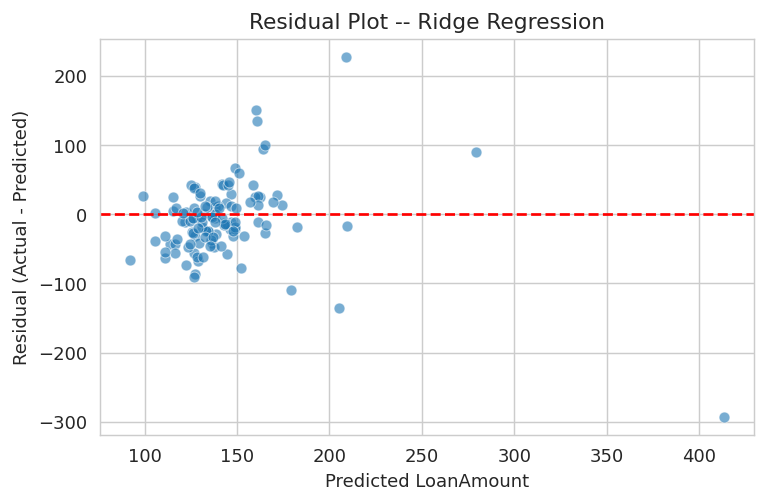
\includegraphics[width=0.55\linewidth]{residual_plot.png}
\caption{Residual plot -- best model (Ridge Regression)}
\end{figure}
\textbf{Inference:} Residuals are not randomly scattered around zero -- they fan out and skew
positive as predicted values increase, a classic heteroscedasticity signature tied directly to
the right-skewed target distribution seen in Figure 1. Taken together, this suggests the constant-variance
assumption of ordinary least squares is violated, and a log-transformed target would likely
produce more homogeneous residuals.

\begin{figure}[H]
\centering
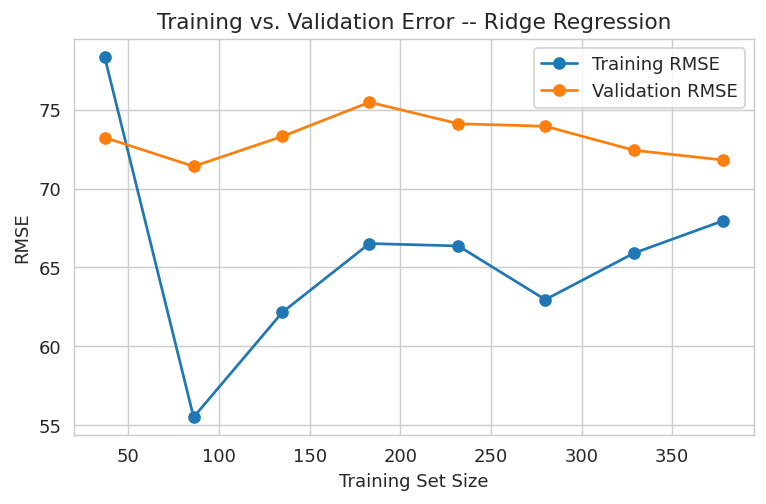
\includegraphics[width=0.55\linewidth]{train_val_error.png}
\caption{Training error vs. validation error (learning curve) -- best model (Ridge Regression)}
\end{figure}
\textbf{Inference:} Training and validation RMSE converge to a similar, persistently high
range ($\approx$55--75) rather than validation error dropping toward training error as more
data is added. This gap-closing-but-high-floor pattern is the signature of \textbf{underfitting
/ high bias} rather than overfitting: the linear feature set does not have enough
capacity to model the target's variance, so more data alone will not substantially help.

\begin{figure}[H]
\centering
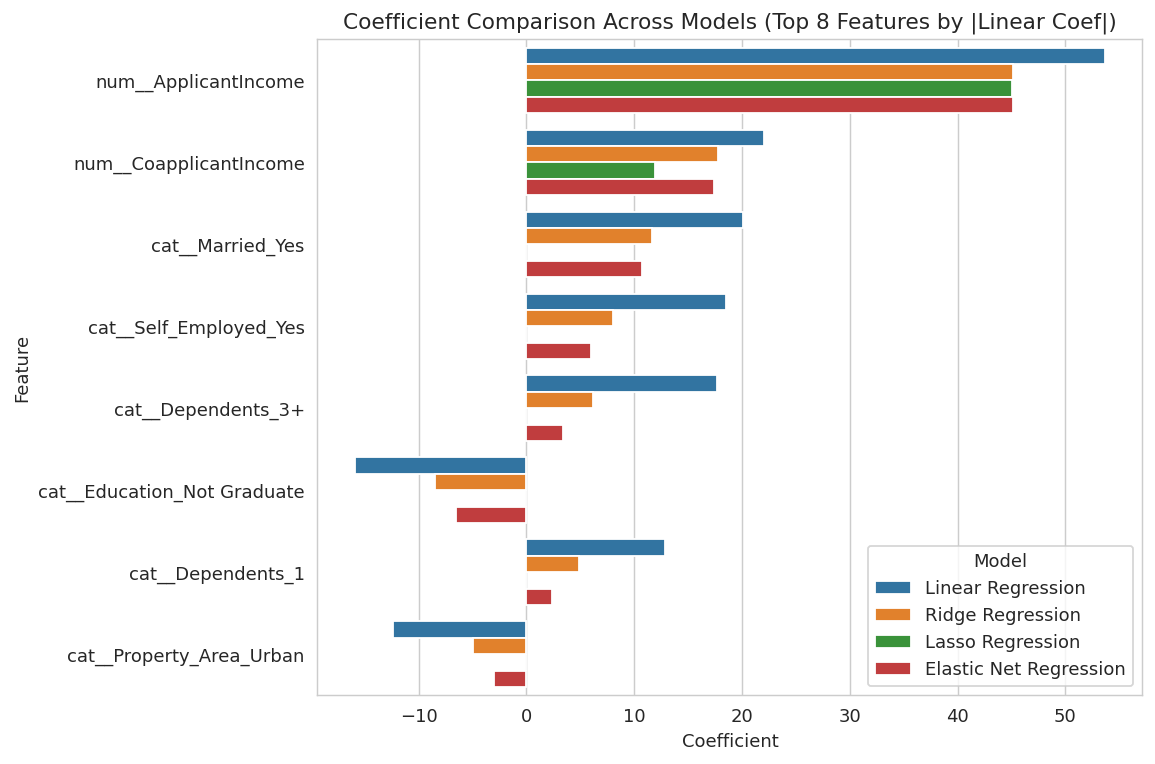
\includegraphics[width=0.75\linewidth]{coefficient_comparison.png}
\caption{Coefficient comparison across models (top 8 features by $|$Linear coefficient$|$)}
\end{figure}
\textbf{Inference:} Ridge shrinks every coefficient toward zero without eliminating any,
Elastic Net shrinks them further while retaining small non-zero weights on most features, and
Lasso is the most aggressive -- it zeroes out Married\_Yes, Self\_Employed\_Yes,
Dependents\_3+, Education\_Not Graduate, Dependents\_1, and Property\_Area\_Urban entirely,
keeping only ApplicantIncome and CoapplicantIncome with non-trivial weight. This is a direct,
visible demonstration of Lasso's feature-selection property versus Ridge's pure shrinkage.

\section{Performance Tables}

\subsection*{Hyperparameter Tuning Summary}
\begin{longtable}{|p{3.2cm}|p{2.6cm}|p{4.5cm}|p{2.2cm}|}
\hline
\textbf{Model} & \textbf{Search Method} & \textbf{Best Parameters} & \textbf{Best CV $R^2$} \\ \hline
\endhead
Ridge Regression & Grid Search & $\alpha = 100$ & 0.3403 \\ \hline
Lasso Regression & Grid Search & $\alpha = 10$ & 0.3151 \\ \hline
Elastic Net Regression & Grid Search & $\alpha = 1$, l1\_ratio $= 0.8$ & 0.3356 \\ \hline
\end{longtable}

\subsection*{Cross-Validation Performance (K = 5, training set)}
\begin{longtable}{|p{3.6cm}|p{2cm}|p{2.3cm}|p{2.3cm}|p{2cm}|}
\hline
\textbf{Model} & \textbf{MAE} & \textbf{MSE} & \textbf{RMSE} & \textbf{$R^2$} \\ \hline
\endhead
Linear Regression & 47.32 & 5590.81 & 74.01 & 0.3015 \\ \hline
Ridge Regression & 44.50 & 5199.02 & 71.80 & 0.3403 \\ \hline
Lasso Regression & 46.45 & 5435.54 & 73.31 & 0.3151 \\ \hline
Elastic Net Regression & 44.45 & 5244.73 & 72.10 & 0.3356 \\ \hline
\end{longtable}

\subsection*{Test Set Performance}
\begin{longtable}{|p{3.6cm}|p{2cm}|p{2.3cm}|p{2.3cm}|p{2cm}|}
\hline
\textbf{Model} & \textbf{MAE} & \textbf{MSE} & \textbf{RMSE} & \textbf{$R^2$} \\ \hline
\endhead
Linear Regression & 36.99 & 3339.92 & 57.79 & 0.0940 \\ \hline
Ridge Regression & 36.84 & 3079.74 & 55.50 & 0.1646 \\ \hline
Lasso Regression & 37.80 & 3181.25 & 56.40 & 0.1370 \\ \hline
Elastic Net Regression & 36.81 & 3087.84 & 55.57 & 0.1624 \\ \hline
\end{longtable}

\textbf{Training time} for all four models was under 10 milliseconds on the 473-row training
set (Linear: 7.2ms, Ridge: 6.7ms, Lasso: 7.0ms, Elastic Net: 6.8ms) -- negligible and not a
practical differentiator at this dataset size.

\textbf{Note on CV vs. test $R^2$:} Across the four models score noticeably higher $R^2$ on
5-fold cross-validation ($\approx$0.30--0.34) than on the single held-out test set
($\approx$0.09--0.16). With only 592 usable samples, a single 119-row test split carries
high variance in its $R^2$ estimate; the CV numbers, averaged over five folds, are the more
stable estimate of true generalization performance.

\subsection*{Effect of Regularization on Coefficients (Top Features)}
\begin{longtable}{|p{4.2cm}|p{2.3cm}|p{2.1cm}|p{2.1cm}|p{2.3cm}|}
\hline
\textbf{Feature} & \textbf{Linear} & \textbf{Ridge} & \textbf{Lasso} & \textbf{Elastic Net} \\ \hline
\endhead
ApplicantIncome & 53.68 & 45.12 & 45.10 & 45.14 \\ \hline
CoapplicantIncome & 22.06 & 17.76 & 11.91 & 17.43 \\ \hline
Married\_Yes & 20.10 & 11.68 & 0.00 & 10.71 \\ \hline
Self\_Employed\_Yes & 18.51 & 8.03 & 0.00 & 5.98 \\ \hline
Dependents\_3+ & 17.64 & 6.20 & 0.00 & 3.43 \\ \hline
Education\_Not Graduate & $-$15.91 & $-$8.47 & $-$0.00 & $-$6.52 \\ \hline
\end{longtable}

\section{Overfitting and Underfitting Analysis}
\begin{itemize}
\item \textbf{Training vs. validation error:} The learning curve (Figure 6) shows training
RMSE (55--78) and validation RMSE (71--75) are already close at small training sizes and stay
close as more data is added -- there is no widening gap that would indicate overfitting.
\item \textbf{Effect of regularization strength:} Grid search selected a large $\alpha=100$
for Ridge, a relatively strong $\alpha=10$ for Lasso, and $\alpha=1$ with a high l1\_ratio of
0.8 for Elastic Net (closer to pure Lasso behaviour). The fact that stronger regularization was
consistently preferred over weaker settings is itself evidence that the baseline linear model
was not egregiously overfitting -- if it were, weak regularization would have already
generalized poorly and the search would have pushed toward much larger $\alpha$ to compensate
for high variance; instead the improvement from regularization is modest (CV $R^2$ 0.30
$\rightarrow$ 0.34), which matches a bias-dominated, not variance-dominated, problem.
\item \textbf{Improvement in generalization after tuning:} Ridge and Elastic Net improved test
RMSE from 57.79 (Linear) to about 55.5, and test $R^2$ nearly doubled (0.094 $\rightarrow$
0.16--0.16). The improvement is real, but not dramatic -- regularization helped, but the
ceiling on all four models' performance is set by the limited linear signal available in the
features, not by uncontrolled overfitting.
\end{itemize}
\textbf{Conclusion of this section:} The main limitation for this dataset is
\textbf{underfitting (high bias)}, not overfitting. Across the four models plateau at a similar,
modest $R^2$, and adding regularization only marginally improves results -- indicating that
the ten available features do not fully explain the variance in LoanAmount, likely because
larger, more influential drivers of loan amount (e.g. property value, requested amount,
lender policy) are not present in this feature set.

\section{Bias--Variance Analysis}
\begin{itemize}
\item \textbf{Bias behaviour of Linear Regression:} Linear Regression has the lowest bias
of the four models (it fits the training data most closely, as seen in its lowest CV RMSE
being only marginally above the regularized models), but this experiment shows even its
unconstrained fit cannot exceed $R^2 \approx 0.30$ on training folds -- indicating the
model family itself (a linear function of these 14 encoded features) has a bias ceiling well
below what the target's variance requires.
\item \textbf{Variance reduction using Ridge and Elastic Net:} Ridge achieved the best CV
$R^2$ (0.3403) and the best test RMSE (55.50) of all four models, and Elastic Net was close
behind -- both shrink coefficient magnitudes (visible directly in Figure 8/Section 6's
coefficient table) which reduces sensitivity to noise in individual training folds, producing
the small but consistent generalization gain seen between the Linear Regression and Ridge
rows of the CV table.
\item \textbf{Feature sparsity effect in Lasso:} Lasso zeroed out 6 of the 14 encoded
features entirely (Married\_Yes, Self\_Employed\_Yes, Dependents\_3+, Education\_Not
Graduate, Dependents\_1, Property\_Area\_Urban), retaining only ApplicantIncome and
CoapplicantIncome with substantial weight. This aggressive sparsity slightly \emph{increased}
bias relative to Ridge (Lasso's CV $R^2$ of 0.3151 is the second-lowest of the four models),
suggesting some of the zeroed categorical features did carry a small amount of genuine
signal that Ridge's softer shrinkage preserved.
\end{itemize}

\section{Observations and Conclusion}
Across the four models converge to a similar, modest performance ceiling (test $R^2$ between 0.09
and 0.16), with \textbf{Ridge Regression} appearing as the best-performing model on both
cross-validation ($R^2=0.3403$) and the held-out test set (RMSE $=55.50$, $R^2=0.1646$),
tuned to $\alpha=100$. Lasso's aggressive feature elimination did not improve performance
over Ridge or Elastic Net, indicating most of the encoded categorical features carry at least
weak signal rather than being pure noise. The Looking at everything together across every diagnostic
(learning curve, CV-vs-test gap, coefficient shrinkage) points to \textbf{underfitting driven
by limited feature information} rather than overfitting: ApplicantIncome and
CoapplicantIncome dominate every model's coefficients, and the available categorical
features (marital status, education, employment, property area) contribute only marginal
additional explanatory power. A practical next step would be engineering additional
features (e.g. income-to-loan-term ratio) or acquiring features more directly tied to the
lender's actual approval formula, rather than further regularization tuning, since
regularization strength is not the binding constraint here.

The trade-off between accuracy and model complexity in this experiment is overall small:
Ridge's mild additional complexity (one tuned hyperparameter) bought a real but modest gain
over the simpler, parameter-free Linear Regression baseline, while Lasso's added complexity
(automatic feature selection) did not translate into a performance advantage on this dataset.

\section{References}
\begin{enumerate}[label={[\arabic*]}]
\item Scikit-learn Developers, ``Linear Models,'' \url{https://scikit-learn.org/stable/modules/linear_model.html}
\item Scikit-learn Developers, ``Tuning the hyper-parameters of an estimator,'' \url{https://scikit-learn.org/stable/modules/grid_search.html}
\item Analytics Vidhya / Kaggle, ``Predict Loan Amount Data,'' \url{https://www.kaggle.com/datasets}
\end{enumerate}

\end{document}
